\documentclass[12pt,AutoFakeBold]{article}%第二个参数解决宋体没有粗体的问题
\usepackage{booktabs}%绘制三线表
\usepackage{fontspec}%控制字体
\usepackage[version=3]{mhchem}%化学反应式
\usepackage{xeCJK}%控制中文字体
\usepackage{latexsym}%绘制特殊数学符号
\usepackage[a4paper]{geometry}%纸张大小和页边距
\usepackage{pdfpages}%插入pdf页面
\usepackage{titlesec}%控制标题格
\usepackage{graphicx, epstopdf}%此处使.eps文件可转化成.pdf并应用自动编号功能
\usepackage[journal=angew]{chemstyle}%此处设置图式的样式
\usepackage{siunitx}%数学模式中使用SI单位
\usepackage{color}%提供颜色支持
\usepackage{listings,xcolor}
\usepackage{amsfonts}

\geometry{left=2.5cm,right=2.5cm,top=2.5cm,bottom=2.5cm}%页边距设置
\setmainfont{Times New Roman}%英文字体
\setCJKmainfont{SimSun}%中文字体
\newfontfamily\arial{Arial}%Arial字体
\XeTeXlinebreaklocale "zh"%中文自动换行
\XeTeXlinebreakskip = 0pt plus 1pt%中文自动换行

\newcommand{\dif}{\mathrm{d}}

\begin{document}
    % cover

    % main body
    \section{问题分析}

    \section{模型设计与计算}
    \subsection{模型的基本假设}
    我们的目标是解出高压油管内部压力$p$与时间$t$的关系,记作
    \begin{equation}
        p=p(t)
    \end{equation}
    \par
    由条件可见,高压油管的内部体$V$不变,由$\rho=\frac{m}{V}$可见,对高压油管内燃油密度造成影响的仅有高压油管内的燃油质量,用微分方程来表达就是
    \begin{equation}
        \dif\rho=\dif\left(\frac{m}{V}\right)=\frac{\dif m}{V}
        \label{eq1}
    \end{equation}
    \par
    首先我们考虑$\dif\rho$和$p$的关系。\par
    根据注1给出的条件,燃油的压力与其密度具有正相关关系,其关系可以用微分方程
    \begin{equation}
         \begin{cases}
            &\dif p=\frac{E}{\rho}\dif\rho\\
            &p_0=\SI{100}{\MPa},\rho_0=\SI{0.850}{\mg\per\cubic\mm}\\
            &E=E(p)
        \end{cases}
        \label{pandrho}
    \end{equation}
    描述,其中$E(p)$由附件3的数据给出,对附件3的数据用MATLAB作图并拟合得到方程,如图\ref{data3}
    \begin{equation}
        E(p)=0.0001p^3-0.001082p^2+5.474p+1532\ \ \ \ (r^2=1.0000)
    \end{equation}
    \begin{figure}[H]
        \centering
        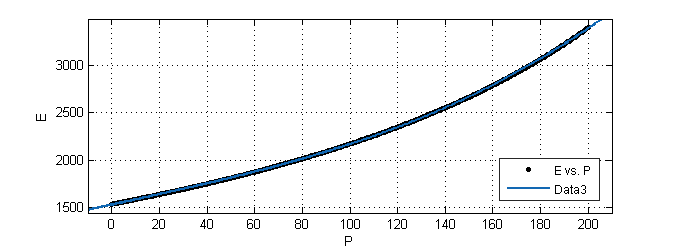
\includegraphics[scale=0.8]{figure/data3.png}
        \caption{燃油弹性模量$E$与压力$p$的非线性拟合结果}
        \label{data3}
    \end{figure}
    由以上的方程我们可以解出关系
    \begin{equation}
        \rho(p)=0.850e^{\int^p_{100}\frac{\dif p}{E(p)}}
        \label{eq2}
    \end{equation}
    \par
    其次,我们再来考虑$\dif m$和$p$与$t$的关系。\par
    $\dif m$由进入和喷出两部分组成。喷出部分对$\dif m$的贡献是时间的函数。单位时间喷出的油量(体积)用函数$Q_{out}(t)$表示,它的解析式在各个小题中有所不同,并且分段可微,所以喷出端造成的$\dif m$可以表述成
    \begin{equation}
        \dif m_{out}=-\rho Q_{out}(t)\dif t
        \label{eq3}
    \end{equation}\par
    进入部分对$\dif m$的贡献也是时间的函数。这个函数含有参数$T$,在上面提及过,它描述了单向阀的开启时间。单位时间进入的油量(体积)用函数$Q_{in}(t)$表示,它的解析式在各个小题中也有所不同,并且分段可微,所以喷出端造成的$\dif m$可以表述成
    \begin{equation}
        \dif m_{in}=\rho Q_{in}(t)\dif t
        \label{eq4}
    \end{equation}\par
    综上,联立方程\ref{eq1}、\ref{eq2}、\ref{eq3}、\ref{eq4},我们可以列出方程
    \begin{equation}
        \frac{\dif p}{E\dif t}=\frac{Q_{in}-Q_{out}}{V}
        \label{maineq}
    \end{equation}\par
    方程\ref{maineq}就是我们对本题建立的基本数学模型。接下来的部分中,我们将根据$Q_{in}(t)$和$Q_{out}(t)$的具体形式,对整个体系最佳$T$值的选择进行讨论。
    
    \subsection{问题1}
    在问题1中$Q_{out}(t)$的形式比较简单,它是由题目中图\ref{inputof1}给出的
    \begin{figure}[H]
        \centering
        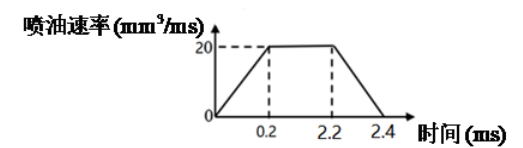
\includegraphics[scale=0.75]{figure/inputof1.png}
        \caption{问题1中的喷油速率}
        \label{inputof1}
    \end{figure}
    写成函数为
    \begin{equation}
        Q_{out}(t)=
        \begin{cases}
            100(t-100k)&100k\leq t\leq 100k+0.2,k\in\mathbb{N}\\
            20&100k+0.2\leq t\leq 100k+2.2,k\in\mathbb{N}\\
            -100(t-100k)+240&100k+2.2\leq t\leq 100k+2.4,k\in\mathbb{N}\\
        \end{cases}
    \end{equation}\par
    在问题1中$Q_{in}(t)$的形式也比较简单,它包括一个参数$T$,描述力单向阀每次开启的时长。我们定义$0-1$变量$\lambda=\lambda(t)$来描述供油处入口的截面积,它的形式为
    \begin{equation}
        \lambda=
        \begin{cases}
            1 & k(T+10)\leq t\leq k(T+10)+T,k\in\mathbb{N}\\
            0 & k(T+10)+T\leq t\leq (k+1)(T+10),k\in\mathbb{N}
        \end{cases}
    \end{equation}
    代入题目中给出的流量公式可得
    \begin{equation}
        Q_{in}(t)=\lambda CA\sqrt{\frac{2(p_h-p)}{\rho_h}}
    \end{equation}\par
    将$Q_{in}(t)$和$Q_{out}(t)$的具体形式代入方程\ref{maineq},发现所得方程是一阶常微分方程,所以尝试用差分法通过计算机进行数值解微分方程,取$\Delta t=\SI{0.01}{ms}$,用Wolfram Mathematica计算并绘制出对应于不同$T$取值$p-t$变化图\ref{ptfigure1}
    \begin{equation}
        \frac{p_{i+1}-p_i}{E(p_i)\Delta t}=\frac{1}{V_0}\left(\lambda CA\sqrt{\frac{2\left(p_h-p_i\right)}{\rho_h}}-Q_{out}(t_i)\right)
    \end{equation}
    \begin{figure}[H]
        \centering
        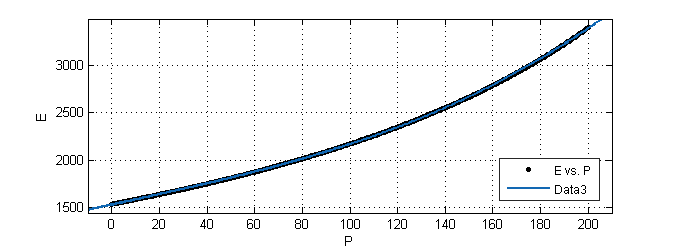
\includegraphics[scale=0.8]{figure/data3.png}%notnow!
        \caption{差分方程数值模拟结果}
        \label{ptfigure1}
    \end{figure}
    利用二分法计算程序可以得到精确到千分位的单向阀开启时长$T=\SI{0.290}{\ms}$。\par
    对于将油管内的压力从\SI{100}{\MPa}提高到\SI{150}{\MPa}的情况,我们可以用同样的差分方程,分别模拟起始压力与\SI{2}{\s}、\SI{5}{\s}和\SI{10}{\s}后的压力差别为\SI{50}{\MPa}时的情况,同样通过二分法可以找出最佳的精确到千分位的单向阀开启时长$T_{2s}=\SI{0.886}{\ms}$、$T_{5s}=\SI{0.713}{\ms}$和$T_{10s}=\SI{0.703}{\ms}$。\par
    \begin{figure}[H]
        \centering
        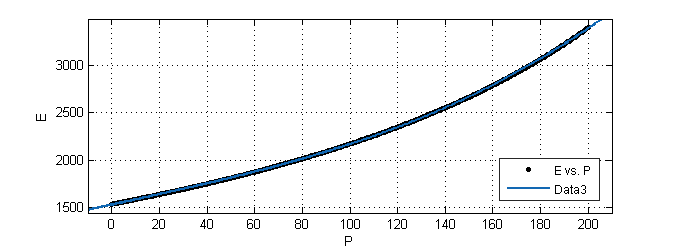
\includegraphics[scale=0.8]{figure/data3.png}
        \caption{调整过程中的压力周期变化}
        \label{adjustpress}
    \end{figure}
    而进过该段时间后,维持\SI{150}{\MPa}所需要的单向阀开启时长为$T_{150}=\SI{0.701}{\ms}$。图\ref{adjustpress}展示了其中一个调整过程中的压力对时间的变化图像。\par
    \paragraph{问题1结论}
    综上所述,将高压油管内的压力尽可能稳定在\SI{100}{\MPa}左右,应该设置单向阀每次开启\SI{0.290}{\ms}。如果要将高压油管内的压力从\SI{100}{\MPa}增加到\SI{150}{\MPa},且分别经过约\SI{2}{\s}、\SI{5}{\s}和\SI{10}{\s}的调整之后稳定在\SI{150}{\MPa}时的情况,对应时长内单向阀应分别先调整为开启$T_{2s}=\SI{0.886}{\ms}$、$T_{5s}=\SI{0.713}{\ms}$和$T_{10s}=\SI{0.703}{\ms}$,随后维持开启时长为$T_{150}=\SI{0.701}{\ms}$,以维持\SI{150}{\MPa}。\par
    
    \section{问题2}
    问题2中$Q_{out}(t)$的形式比较复杂。\par
    首先我们定义等效面积函数$B(t)$,用来描述针阀运动过程中喷油嘴喷孔的等效面积。由简单的几何计算可知,它的形式如下。
    \begin{equation}
        B(t)=\pi\left(\left(\frac{d_B}{2}+h(t)\tan9^\circ\right)^2-\left(\frac{d_B}{2}\right)^2\right)
    \end{equation}\par
    但是,当针阀上升到一定高度时,等效面积函数值会超过喷嘴的面积,此时喷油能力转而由喷嘴的面积限制,为了不改变$B(t)$的表达形式,我们定义了等效升程函数$h(t)$,它表示针阀的等效升程,由题目附件2给出的数据拟合,并按照前述进行修正得到,其图形和拟合结果如下
    \begin{equation}
        h(t)=
        \begin{cases}
            \frac{0.5342(t-100k)^2-0.04835(t-100k)+0.000726}{(t-100k)^2-0.7362(t-100k)+0.1716}&100k\leq t\leq 100k+0.3309,k\in\mathbb{N}\\
            1.1532&100k\leq t+0.3309\leq 100k+2.1213,k\in\mathbb{N}\\
            \frac{0.5358(t-100k)^2-2.576(t-100k)+3.096}{(t-100k)^2-4.163(t-100k)+4.368}&100k+2.1213\leq t\leq 100k+2.45,k\in\mathbb{N}\\
            0&100k+2.45\leq t\leq 100(k+1),k\in\mathbb{N}\\      
        \end{cases}
    \end{equation}
    \begin{figure}[H]
        \centering
        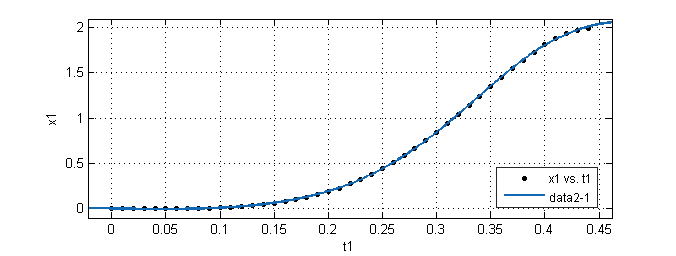
\includegraphics[scale=0.8]{figure/data21.png}
        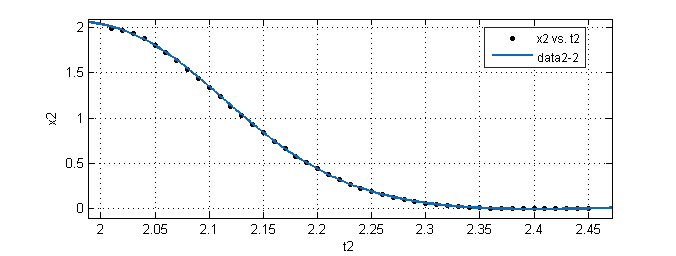
\includegraphics[scale=0.8]{figure/data22.png}
        \caption{针阀升程}
        \label{zhenfa}
    \end{figure}
    由于高压油管内的油压远高于大气压,所以我们可以忽略喷油嘴外的压强,即$\Delta p\approx p$,由此$Q_{out}(t)$就可以被写成
    \begin{equation}
        Q_{out}(t)=CB\sqrt{\frac{2p}{\rho}}
    \end{equation}\par
    再来看$Q_{in}$的表达形式,它形式上与上一题类似,如方程\ref{qin2}(以下下标为$h$的项均为油泵油缸的性质)
    \begin{equation}
        Q_{in}(t)=\delta CA\sqrt{\frac{2(p_h-p)}{\rho_h}}
        \label{qin2}
    \end{equation}
    其中$0-1$变量$\delta$定义如下
    \begin{equation}
        \delta=
        \begin{cases}
            1&p_h\geq p\\
            0&p_h<p\\
        \end{cases}
    \end{equation}\par
    下面我们来求油缸内压力$p_h$的表达式。油缸的体积可以表示为时间$t$的周期函数
    \begin{equation}
        V_h(t)=20+(R_{up}-R(\theta(t)))\pi\left(\frac{5}{2}\right)^2
    \end{equation}
    其中$R_{up}$为凸轮位于上止点时的极径,由题目给出,为\SI{0.5}{\MPa},$R(\theta)$的表达式由题目附件1给出,$\theta(t)$的表达式如下,为了计算方便,我们把时刻$t=0$的相位设置为下止点,也就是$\theta = \pi$。
    \begin{equation}
        \theta(t)=\omega t+\pi -2k\pi,k\in\mathbb{N},\theta(t)\geq0
    \end{equation}
    当油泵活塞运行到下止点时,油泵吸慢了油,并不再把油返回低压油路,所以我们可以在油泵位于下止点时直接给定一个初值$p_0=\SI{0.5}{\MPa}$,对每一个周期都是这样。\par
    考虑油泵油缸的质量守恒,可以得到下面的方程。
    \begin{equation}
        \frac{\dif m_h}{\dif t}=-Q_{in}\rho
        \label{highmaineq}
    \end{equation}
    又由密度的定义$m_h=\rho_hV_h$微分得到
    \begin{equation}
        \dif m_h=\rho_h\dif V_h+V_h\dif\rho_h
        \label{higheq2}
    \end{equation}
    将方程\ref{pandrho}、\ref{highmaineq}、\ref{higheq2}联立,加入初值条件,可以整理得到
    \begin{equation}
        \begin{cases}
            \frac{\dif p_h}{E(p_h)\dif t}=\frac{1}{V_h}\left(-Q_{in}\frac{\rho}{\rho_h}-\frac{\dif V_h}{\dif t}\right)\\
            p_h(\frac{2k\pi}{\omega})=0.5,k\in\mathbb{N}
        \end{cases}
        \label{highmaineq2}
    \end{equation}\par
    在高压油泵供油的过程中我们可以用方程\ref{highmaineq2}去描述它的情况。这个方程的形式和刚才对高压油管的建模模型——方程\ref{maineq}形式很相似,也就是我们可以把高压油泵的油缸视作另一个高压油管,活塞对它的压缩可以视作$Q_{in}$,而向高压油管供油可以视作$Q_{out}$,当然此时$V$是变量,所以不可以直接代入。\par
    同时,根据方程\ref{maineq}我们可以写出高压油管的方程
    \begin{equation}
        \frac{\dif p}{E\dif t}=\frac{Q_{in}-Q_{out}}{V}
        \label{maineq2}
    \end{equation}
    联立方程\ref{maineq2}、\ref{highmaineq2}并使用和问题1中相似的差分方程计算
    \begin{equation}
        \begin{aligned}
            &\frac{p_{h\ i+1}-p_{h\ i}}{E(p_{h\ i})\Delta t}=\frac{1}{V_h(t_i)}\left(-\delta CA\sqrt{\frac{2\left(p_h-p_i\right)}{\rho_h}}\frac{\rho}{\rho_h}-\frac{\dif V_h}{\dif t}\right)\\
            &\frac{p_{i+1}-p_i}{E(p_i)\Delta t}=\frac{1}{V_0}\left(\delta CA\sqrt{\frac{2\left(p_h-p_i\right)}{\rho_h}}-Q_{out}(t_i)\right)\\
            &p_h(\frac{2k\pi}{\omega})=0.5,k\in\mathbb{N}
        \end{aligned}
    \end{equation}

    % appendix
        
\end{document}